%TCIDATA{Version=5.00.0.2570}
%TCIDATA{LaTeXparent=0,0,Presentation-CAFE-displacement-subdoc.tex}
% $Id: Presentation-subdoc-access.tex 1766 2015-11-11 19:14:54Z lv39 $
% $URL: https://forge.cornell.edu/svn/repos/lv39_papers/BigThinkPresentations/UQAM2015/Presentation/Presentation-subdoc-access.tex $
\section{Context}


\begin{frame}
\frametitle{Economic analysis}
	\centering
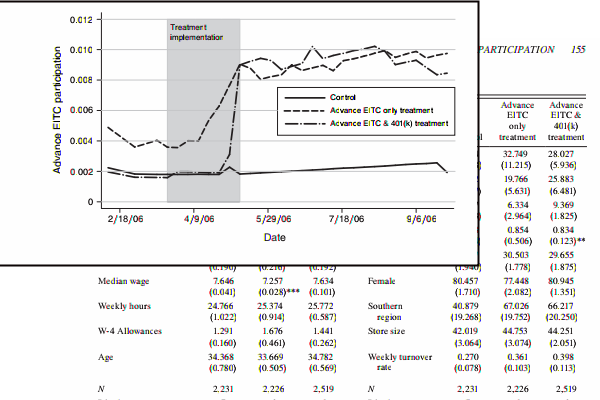
\includegraphics[width=0.9\textwidth]{Selection_119.png}
\end{frame}


\begin{frame}
\frametitle{The preponderance of public-use data}
\begin{block}{Microdata}
\begin{quote}
	``... paper uses data from the Current Population Survey...''
\end{quote}
\end{block}

\pause
\begin{block}{Macrodata}
	\begin{quote}
		``We use data downloaded from the Bureau of Economic Analysis...''
	\end{quote}
\end{block}

\end{frame}

% disaster: http://filmsplusmovies.com/wp-content/uploads/2013/08/Best-Natural-Disaster-Movies-Of-Hollywood.jpg

\begin{frame}
\centering
	
\includegraphics{temptation.jpg}% source:

	\tiny \href{http://www.bridgesofgraceucc.org/}{source} %http://www.bridgesofgraceucc.org/wp-content/uploads/2011/03/temptation.jpg
\end{frame}


\begin{frame}
\frametitle{Yielding...}
\begin{block}{Administrative data}
\begin{quote}
 ``Our analysis draws on administrative records from the Detroit Work First program
linked with unemployment insurance (UI) wage records for the State of
Michigan'' 

\tiny \href{http://doi.org/10.1257/app.2.3.96}{Autor/Houseman doi:10.1257/app.2.3.96}
\end{quote}
\end{block}
\pause
\begin{block}{Administrative data}
\begin{quote}
	``confidential student-level panel
dataset provided by the School Board of Alachua County in Florida'' 

\tiny \href{http://doi.org/10.1257/app.2.1.211}{Carrel and Hoekstra doi:10.1257/app.2.1.211}

\end{quote}\end{block}
\end{frame}


\begin{frame}
\frametitle{... yielding...}
\begin{block}{Proprietary data}
\begin{quote}
	``This field experiment was made possible by the collaboration of a large-scale,
	nationwide firm in the retail sector. ''
	
	\tiny \href{http://doi.org/10.1257/app.2.2.147}{Damon doi:10.1257/app.2.2.147}
\end{quote}
\end{block}
\end{frame}



\begin{frame}
\frametitle{The Death Knell for Public-use Data}

\centering
	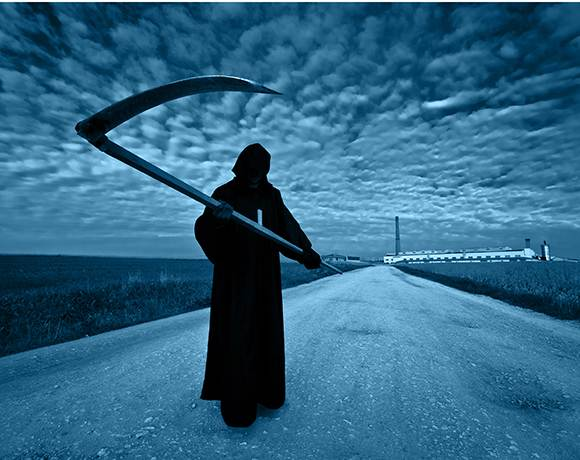
\includegraphics[width=.9\textwidth]{deathknell.jpg}% source: http://cdn.ttgtmedia.com/rms/onlineImages/ciomid_trends_2012_08.jpg

\end{frame}

\begin{frame}
	\frametitle{The Death Knell for Public-use Data}
\begin{itemize}
	\item Sounded by young scholars pursuing research
	programs that mandate inherently identifiable data:
			\begin{itemize}
				\item Geospatial relations,
				\item Exact genome data,
				\item Networks of all sorts,
				\item Linked administrative records
			\end{itemize}
			\item These researchers acquire authorized, generally unfettered, restricted access to the
			confidential, identifiable data and perform their analyses in secure
			environments.
\item But...

\end{itemize}
\end{frame}

\begin{frame}
%	\frametitle{The provenance problem}
	\begin{beamercolorbox}[sep=8pt,center]{title}
		\usebeamerfont{title} ...they don't leave behind the scientific trail that has
		made public-use files so important.
	\end{beamercolorbox}
\end{frame}


\begin{frame}
	\frametitle{Replication of research results}
	\begin{block}{Critical element of science}
		\begin{itemize}
			\item Replication of methods, data inputs, computational environment is a critical element of the scientific approach
			\item Journals, funding agencies (in the U.S.) have been moving to making archiving of inputs to scientific results more robust, even mandatory
		\end{itemize}
	\end{block}
\end{frame}


\begin{frame}
\frametitle{The problem}
\begin{block}{Good intentions, costly access}
\begin{quote}
	``researchers could submit programs that [...] research assistants
	would run. Alternatively, researchers wishing to work directly with the data could come and
	work on the Institute's premises. ''
\end{quote}
\end{block}
\pause
\begin{block}{Uncertain access}
\begin{quote}
	``Data [...] is proprietary and owned by the Alachua
County, Florida School District. The corresponding author [...] holds the deidentified
dataset [...] and will provide copies to
authors who receive written permission from the Alachua County Public Schools.''
\end{quote}
\end{block}
\pause
\begin{block}{No access}
\begin{quote}
	Some do not provide any information on access.	
\end{quote}
\end{block}
\end{frame}




\begin{frame}
	\frametitle{Not a new problem}
	\begin{columns}
	\begin{column}{.7\textwidth}
	\begin{block}{Econometrica}
		``In its first issue, the editor of Econometrica (1933), Ragnar Frisch, noted
		the importance of publishing data such that readers could fully explore
		empirical results.  Publication of data, however, was discontinued early in
		the journal's history.  [...]  The journal arrived full-circle in late 2004 when Econometrica
		adopted one of the more stringent policies on availability of data and
		programs.
	\end{block}
	\tiny \href{http://www.econometricsociety.org/submissions.asp\#4}{http://www.econometricsociety.org/submissions.asp\#4} as cited in \href{http://research.stlouisfed.org/wp/2005/2005-014.pdf}{Anderson et al (2005)}
	\end{column}
	\begin{column}{.3\textwidth}
\href{http://www.jstor.org/stable/i332704}{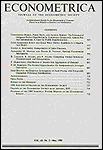
\includegraphics[width=\textwidth]{econometrica-vol1.png}}
	\end{column}
\end{columns}
\end{frame}

\begin{frame}
	\frametitle{Problem will become worse}
	\begin{block}{Increased use of restricted-access data}
\begin{itemize}
			\item Archiving (curation) of input data is complicated
			\item Knowledge discovery is complicated
		\end{itemize}
	\end{block}
\end{frame}
\begin{frame}
	\frametitle{Decline in the use of classic public-use data}
	\centering
	%\includepdf[pages={1-2}]{Chetty-1-2-Slides.pdf}
	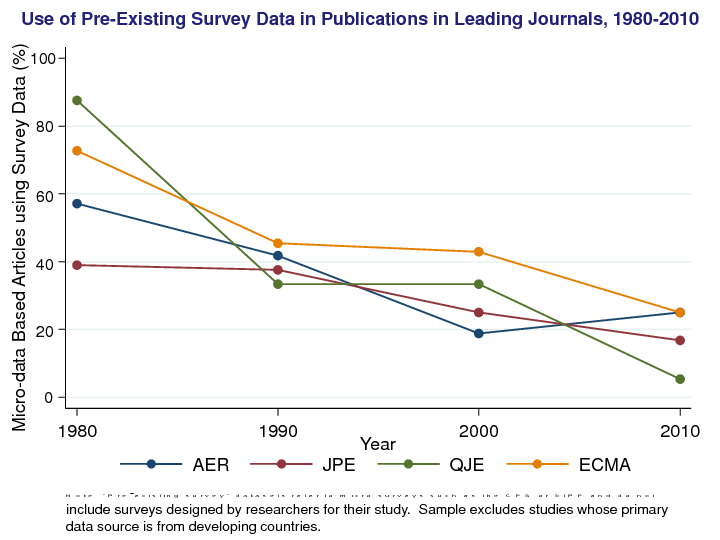
\includegraphics[width=0.7\paperwidth]{ChettySlide1}
\end{frame}

\begin{frame}
	\frametitle{Increase in the use of administrative data in economics}
	\centering
	%\includepdf[pages={1-2}]{Chetty-1-2-Slides.pdf}
	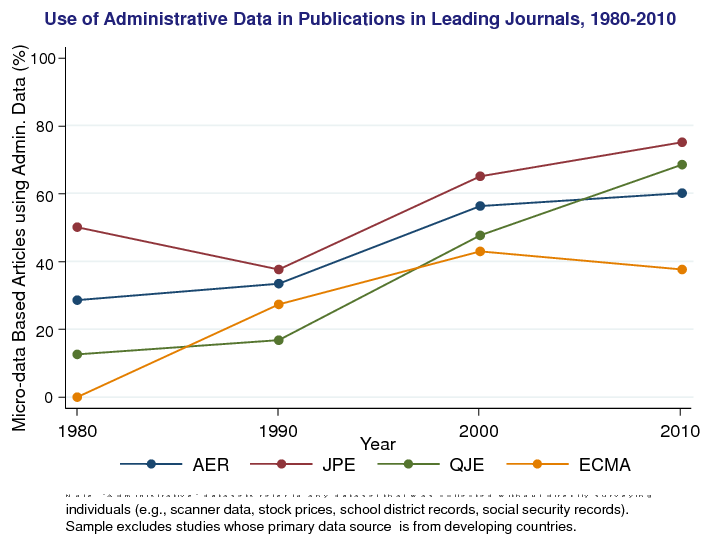
\includegraphics[width=0.7\paperwidth]{ChettySlide2}
\end{frame}


\begin{frame}
\frametitle{Results from the LDI Replication Lab}
	\begin{block}{Undergraduate research team}
		\begin{itemize}
			\item Census of articles in the American Economic Journal: Applied Economics (2010, 2011, 2013)
			\item Each article is analyzed for availability of replication archive (as required by journal!) 
			\item If data and programs are available, reproducibility is tested. 
		\end{itemize}
	\end{block}
\end{frame}

% extract from Replication.Rnw

\begin{frame}
\frametitle{Some very preliminary results}
	
	\centering
	\begin{table}[!htbp] \centering 
		\caption{Replication Success} 
		\label{} 
		\begin{tabular}{@{\extracolsep{5pt}} ccccc} 
			\\[-1.8ex]\hline 
			\hline \\[-1.8ex] 
			& Yes & No & Partial & Sum \\ 
			\hline \\[-1.8ex] 
			2010 & $10$ & $19$ & $6$ & $35$ \\ 
			2011 & $12$ & $20$ & $4$ & $36$ \\ 
			2013 & $15$ & $12$ & $11$ & $38$ \\ 
			\hline \\[-1.8ex] 
			
			\bf		Total &\bf $37$ &\bf $51$ &\bf $21$ &\bf $109$ \\ 
			\hline \\[-1.8ex] 
		\end{tabular} 
	\end{table} 
\end{frame}

\begin{frame}
\frametitle{Some very preliminary results}
	% Table created by stargazer v.5.2 by Marek Hlavac, Harvard University. E-mail: hlavac at fas.harvard.edu
	% Date and time: Mon, Nov 09, 2015 - 09:22:20 PM
	\centering \small
	\begin{table}[!htbp] 
		\caption{Reason for Replication Failure} 
		\label{} 
		\begin{tabular}{@{\extracolsep{5pt}} cccccc} 
			\\[-1.8ex]\hline 
			\hline \\[-1.8ex] 
			& Missing  & Corrupted  & Code  & Missing &  \\ 
			& Data     & Data       & Error & Code    & Sum \\ 
			\hline \\[-1.8ex] 
			2010 & $15$ & $1$ & $1$ & $2$ & $19$ \\ 
			2011 & $15$ & $1$ & $1$ & $3$ & $20$ \\ 
			2013 & $12$ & $0$ & $0$ & $0$ & $12$ \\ 
			\hline \\[-1.8ex] 
			\bf Total &\bf $42$ &\bf $2$ &\bf $2$ &\bf $5$ &\bf $51$ \\ 
			\hline \\[-1.8ex] 
		\end{tabular} 
	\end{table} 
\end{frame}


\begin{frame}
\frametitle{Some very preliminary results}
	\centering
	% Table created by stargazer v.5.2 by Marek Hlavac, Harvard University. E-mail: hlavac at fas.harvard.edu
	% Date and time: Tue, Nov 10, 2015 - 01:24:18
	\begin{table}[!htbp] \centering 
		\caption{Reason for Missing Data} 
		\label{} 
		\begin{tabular}{ ccccccc} 
			\\[-1.8ex]\hline 
			\hline \\[-1.8ex] 
		&\multicolumn{3}{c}{Administrative}&\multicolumn{2}{c}{Private} &  \\ 
		\cline{2-4}\cline{5-6}
		&  local &  National &  Regional &  Commercial &  Other & Sum \\ 
		\hline \\[-1.8ex] 
		2010 & $2$ & $8$ & $0$ & $4$ & $3$ & $17$ \\ 
		2011 & $2$ & $8$ & $4$ & $1$ & $0$ & $15$ \\ 
		2013 & $2$ & $2$ & $1$ & $4$ & $2$ & $11$ \\ 
			\hline \\[-1.8ex] 
		Total & $6$ & $18$ & $5$ & $9$ & $5$ & $43$ \\ 
			\hline \\[-1.8ex] 
		\end{tabular} 
	\end{table} 
\end{frame}


\begin{frame}
	\frametitle{Some very preliminary results}
% Table created by stargazer v.5.2 by Marek Hlavac, Harvard University. E-mail: hlavac at fas.harvard.edu
% Date and time: Tue, Nov 10, 2015 - 01:24:18
\begin{table}[!htbp] \centering 
	\caption{Type of Access to Confidential Data} 
	\label{} 
	\begin{tabular}{ cccccc} 
		\\[-1.8ex]\hline 
		\hline \\[-1.8ex] 
		&  &\multicolumn{2}{c}{Informal} & No  &  \\ 
		& Formal & w/ Commitment & w/o Commitment &  Info & Sum \\ 
		\hline \\[-1.8ex] 
		2010 & $2$ & $3$ & $9$ & $3$ & $17$ \\ 
		2011 & $2$ & $0$ & $10$ & $3$ & $15$ \\ 
		2013 & $1$ & $2$ & $8$ & $0$ & $11$ \\ 
		\hline \\[-1.8ex] 
	\bf	Total & $5$ & $5$ & $27$ & $6$ & $43$ \\ 
		\hline \\[-1.8ex] 
	\end{tabular} 
\end{table} 
		\end{frame}



\begin{frame}
	\frametitle{Not limited to one journal}
	\begin{block}{NIH-funded research}
		\begin{itemize}
			\item article is open-access
			\item not clear about data access
		\end{itemize}
	\end{block}
\end{frame}

  \tikzset{
  	arr/.style={->,blue,very thick},
  	lbl/.style={draw,blue,very thick},
  	shadowed/.style={preaction={transform canvas={shift={(2pt,-1pt)}},draw=gray,very thick}},
}
\begin{frame}
	\frametitle{A small anonymous example}
   \begin{tikzpicture}
   \node[draw=none,drop shadow={shadow scale=0.97,
   top color=black,bottom color=gray,
                          shadow xshift=3pt,
                          shadow yshift=-2pt,
   opacity=0.9}]
    at (1,1) {\fcolorbox{black}{white}{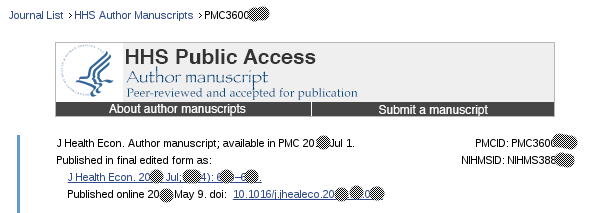
\includegraphics[scale=0.5]{Selection_031}}}; \pause
%
      \node[draw=none,drop shadow={shadow scale=0.95,
      	top color=black,bottom color=gray,
      	shadow xshift=3pt,
      	shadow yshift=-2pt,
      	opacity=0.9}]
      at (1,1) {\fcolorbox{black}{white}{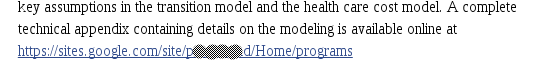
\includegraphics[scale=0.5]{Selection_030}}};
\pause
      \node[draw=none,drop shadow={shadow scale=0.93,
      	top color=black,bottom color=gray,
      	shadow xshift=3pt,
      	shadow yshift=-2pt,
      	opacity=0.9}]
      at (1,1) {\fcolorbox{black}{white}{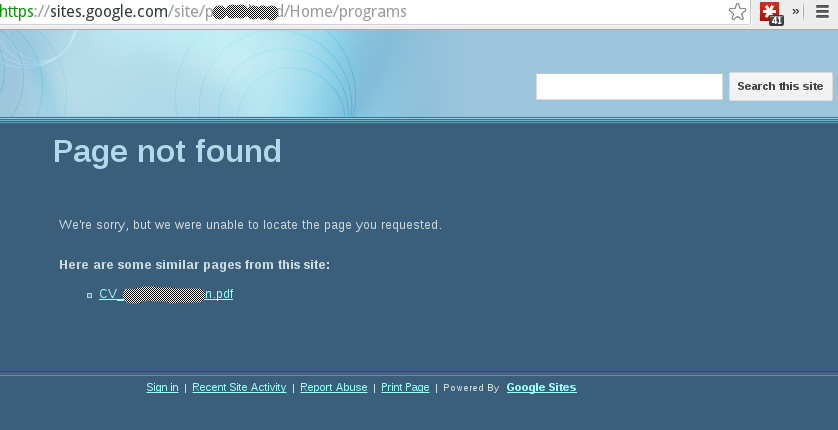
\includegraphics[scale=0.25]{Selection_032}}};
\pause
\node[draw=none,drop shadow={shadow scale=0.93,
	top color=black,bottom color=gray,
	shadow xshift=3pt,
	shadow yshift=-2pt,
	opacity=0.9}]
at (1,1) {\fcolorbox{black}{white}{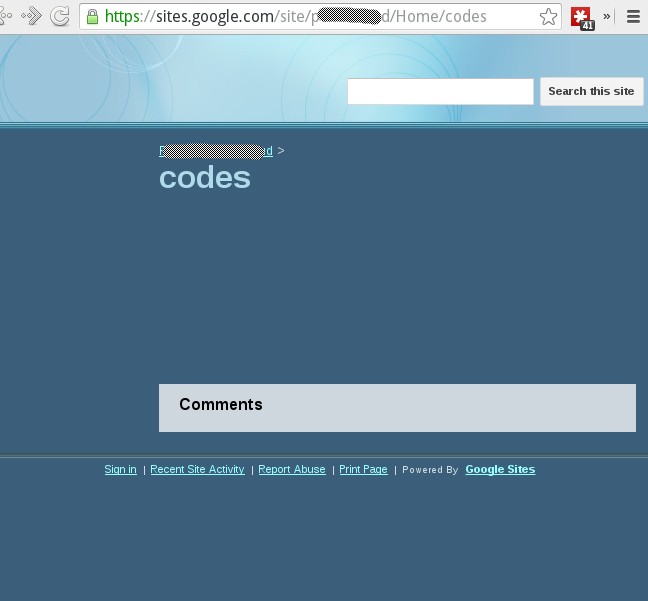
\includegraphics[scale=0.25]{Selection_029}}};
   \end{tikzpicture}

\end{frame}

\begin{frame}
	\frametitle{Not limited to economics}
	\begin{block}{Nature, 2012}
		``Many of the emerging `big data' applications come from private sources that are inaccessible to other researchers. The data source may be hidden, compounding problems of verification, as well as concerns about the generality of the results.''\\
	\end{block}
	{\tiny (Huberman, Nature 482, 308 (16 February 2012) \href{http://dx.doi.org/10.1038/482308d}{doi:10.1038/482308d})}
	\begin{block}{Other domains}
		\begin{itemize}
			\item Biology (genetics data, chemical compounds)
			\item Computer science (search records, single-firm examples)
		\end{itemize}
	\end{block}
\end{frame}


\begin{frame}
	\centering
	
\includegraphics[width=\textwidth]{Best-Natural-Disaster-Movies-Of-Hollywood.jpg}
\end{frame}



\begin{frame}
\frametitle{A program}
%\begin{block}{Broadening access}
%	\begin{itemize}
%		\item Public-use data is the ultimate decentralized computation
%		\item Current limits of the infrastructure
%		\item Infrastructure
%	\end{itemize}
%\end{block}


\begin{block}{Allowing for easier documentation of provenance}
\begin{itemize}
	\item Better documentation about confidential data
	\item Solving the reproducibility problem
\end{itemize}
\end{block}

\begin{block}{Making data more accessible}
	\begin{itemize}
		\item New disclosure limitation techniques
		\item New data access models
	\end{itemize}
\end{block}
\end{frame}


%%% Local Variables:
%%% mode: latex
%%% End:
